\chapter{Background and Related Work}
\label{sec:background}

% Source notes: Vault/wiki (concepts: Prefill and Decode, KV Cache, On-Device Inference, Apple Silicon and MLX, Energy of
% LLM Inference, decision model Models, Letter-Token Readout, Laya, Decision-Model Benchmarks, Groundedness Verification,
% Hallucination Detection, Calibration, Verbalised vs Logit Confidence, Fine-tuning Instability and Seeds).

This chapter reviews the work on which GroundOne builds and the work against which it is compared. The cost of inference
on a local device, from which the design follows, was already treated in Chapter~\ref{sec:local}. The chapter starts
from decision models, that is, from the idea of reading the decisions of a language model instead of having it generate
them, and from their rapidly growing ecosystem. It then turns to the problem of hallucination in retrieval-augmented
generation (RAG) and to the methods that verify answers against their sources. It closes with calibration, with
parameter-efficient fine-tuning and with the gap that this thesis sets out to fill.

\section{Decision models}
\label{sec:bg-systemone}

The term \emph{System One model} was introduced by TypeSafe with Jev, a model offered as a hosted service. Jev answers
closed questions about a given state, that is, about the context supplied in the request, and returns typed outputs,
such as a boolean, a choice among options or a score, without generating text~\cite{typesafe2026jev}. The name evokes
the fast, intuitive thinking described by Kahneman, as opposed to deliberate reasoning. The vendor reports latencies
ranging from tens to hundreds of milliseconds and large savings with respect to generative judges. These figures,
however, remain vendor claims, and the architecture is not disclosed.

The open implementations that followed differ in how they produce the probabilities, and three families can be
identified. The most common one presents the question as a multiple choice and keeps the head of the language model,
that is, the final layer that assigns a score to every token of the vocabulary: the decision is read from the logits of
the option letters, at the position where the model would write the answer. SemIf applies this readout to a 4B-parameter
model kept frozen, that is, without modifying its weights, and reports that 21 criteria about one document are answered
in about one second; the best generative baseline able to produce valid JSON, by contrast, takes more than five
seconds~\cite{semif}. Rizzo-Flow, unlike SemIf, fine-tunes a 4B model with LoRA on typed decisions and exposes the same
interface as Jev. Its authors report that fine-tuning improves both its accuracy and its calibration~\cite{rizzoflow}.
This is the general-purpose decision model used as a baseline in this thesis.

The second family encodes the state and each candidate answer separately, and compares their embeddings, that is, the
numerical vectors that represent each text. Contrastive Language Models, which belong to this family, are very fast
when the candidates are numerous and reusable. In the comparison reported by the authors themselves, however, they agree
with Jev's decisions much less than a model in which state and candidate interact~\cite{kwok2026clm}. The third family
uses small encoders\footnote{An \emph{encoder} is a transformer in which every token attends to all the others, both
those that precede it and those that follow it. It produces a representation of the text instead of generating text, as
BERT and the models derived from it do. The \emph{mask token} is a special token that, during pre-training, takes the
place of the words the model has to reconstruct.} with a dedicated decision head. Laya, for example, is built on a
ModernBERT encoder of about 400M parameters and assigns a score to each option at the corresponding mask token. The
questions of a request are evaluated in a single call, grouped into a batch, but each of them is encoded together with
its own copy of the context~\cite{convai2026laya,azizi2026labels}.

The evidence supporting these systems is uneven. Most of it comes from the authors themselves, often on a single machine
and on a single benchmark. Independent evaluations are recent and less favourable to small open models. An evaluation of
Jev on 37 datasets finds well calibrated the probabilities that the model assigns to choices among options. Binary
probabilities, instead, rank examples well but are poorly positioned with respect to a fixed threshold of 0.5. The same
study reports for Jev a mean balanced accuracy\footnote{\emph{Balanced accuracy} is the mean, computed over the classes,
of the recall, that is, of the fraction of examples of each class that are classified correctly. Unlike plain accuracy,
it does not reward a model that always predicts the most frequent class: a constant predictor obtains 0.5 in the binary
case (50 when expressed as a percentage, as here) and about 0.33 with three classes.} of 78.6 on
LLM-AggreFact~\cite{deusser2026jev}. An independent reproduction of Laya observes a calibration different from the
declared one and a strong dependence on a calibration temperature estimated on the target
data~\cite{nandakishore2026laya}. A benchmark built on contrastive pairs, that is, on nearly identical decisions that
differ in a single decisive detail, places small open models far below Jev~\cite{yong2026decidebench}. Finally, it has
been shown that, when the label of an option and its definition conflict, typed decision models follow the label rather
than the definition~\cite{azizi2026labels}.

The ecosystem, meanwhile, is growing rapidly. On 9 October 2026 the Hugging Face hub officially introduced a tag
dedicated to these \emph{decision models}~\cite{hf2026decisionmodels}. The following day the tag already grouped about
1{,}500 models, published by about 600 authors and of very uneven quality. This thesis uses the term \emph{decision
model}, adopted by the ecosystem; \emph{System One} remains the name with which TypeSafe introduced the category, and in
what follows it appears only as the name of the Jev-compatible interface.

A few weeks after the release of Jev, established organisations also published their own open decision models.
Cloudflare's Clef adds a dedicated decision head to a decoder and answers all the questions with a single forward pass
over the state: this is the architecture that had only been hypothesised for Jev~\cite{cloudflare2026clef}. Liquid AI's
d1-3B reads the decision from a restricted set of answer letters, with a 3B model whose state is shared by all the
questions~\cite{liquid2026d1}. Perplexity, finally, fine-tunes a 27B model with a head on the
letters~\cite{perplexity2026decider}. A community leaderboard, the Decision Index, evaluates these models on a common
battery of public benchmarks, including RAGTruth evaluated at the level of the whole answer~\cite{decisionindex2026}.
The results draw a sharp line. General-purpose decision models with fewer than one billion parameters barely beat the
trivial baseline on RAGTruth, and only models with tens of billions of parameters reliably detect hallucinated answers.

The studies on Jev add three observations. Its probabilities are calibrated when aggregated over many tasks, but not on
a single task. Thresholds and temperatures have to be estimated on the target workload~\cite{guo2026justaskjev,li2026jevjudge}.
Finally, choosing the threshold through a lower confidence bound makes it safer to put into production a judge that
returns only decisions~\cite{li2026jevjudge}. Runtimes have adapted as well: llama.cpp now natively supports the System
One interface~\cite{llamacpp}. None of these models, however, is specialised in groundedness, that is, in the adherence
of the answer to the document. Nor does any of them report results of three-class, sentence-level verification on the
benchmarks used in this thesis.

The letter readout has also been studied outside the decision-model literature, in multiple-choice question answering.
Here two ways of obtaining the answer of an instruction-tuned model can be compared: reading which letter has the highest
probability as the first token, or letting the model write out the answer in full. The two answers often do not
coincide~\cite{wang2024myanswerc}. The readout, moreover, favours particular option identifiers, such as certain
letters, and this bias can be estimated and removed~\cite{zheng2024mcq}. Both results concern models used zero-shot.
They suggest that a letter readout, if it is to serve as a decision, needs to be trained, calibrated or both. Moreover,
no open decision model has been specialised in groundedness verification and then compared, under controlled conditions
and on the same hardware, with generative judges, with specialised verifiers and with general-purpose decision models,
one of them of the same size.

\section{Retrieval-augmented generation and hallucination}
\label{sec:bg-rag}

Retrieval-augmented generation (RAG) gives a language model access to documents on which it was not trained: a
retriever selects the passages relevant to the question, and the model writes the answer with these passages in its
context~\cite{lewis2020rag}. It is the standard approach for building assistants over private documents, and it can run
entirely on a local machine. It does not, however, eliminate hallucinations. Surveys of the literature distinguish two
types of error. Errors of \emph{factuality} are measured against world knowledge, errors of \emph{faithfulness} against
the input or the context given to the model~\cite{huang2025hallucination}. A RAG answer, in particular, can be
unfaithful to the very passages it received, by contradicting them or by adding information that they do not contain.

RAGTruth documents how frequent this is. The dataset collects about 18{,}000 answers, written by six language models on
three RAG-style tasks, and annotates in them, with character-level precision, the spans of text that conflict with the
context or are not supported by it~\cite{niu2024ragtruth}. RAGTruth's distinction between conflicting content and
baseless content corresponds to the classes \emph{contradicted} and \emph{not mentioned} adopted in this thesis.

\section{Groundedness verification}
\label{sec:bg-verification}

Verifying an answer against its source is a problem closely related to natural language inference (NLI). In NLI the
task is to establish whether a premise implies a hypothesis (entailment), contradicts it or is neutral with respect to
it. Large NLI datasets provide training data: MultiNLI~\cite{williams2018mnli} and ANLI~\cite{nie2020anli}, the latter
built adversarially, that is, by collecting examples written on purpose to fool the models of the time.
VitaminC~\cite{schuster2021vitaminc} adds contrastive pairs, in which a minimal revision of a Wikipedia sentence flips
the verdict: the model is thus forced to look at the precise fact rather than at word overlap.

Applying these models to long generated texts requires decomposing them. SummaC splits both the document and the summary
into sentences and aggregates the inference scores computed sentence by sentence~\cite{laban2022summac}. FActScore,
instead, decomposes long generations into atomic facts and verifies them one by one~\cite{min2023factscore}.
Sentence-level verification, adopted by GroundOne, lies between a single score for the whole answer and the
decomposition into atomic facts. Sentences are the natural units of an answer, the user can act on a flagged sentence,
and the number of decisions grows with the length of the answer.

In practice two families of verifiers prevail. The first is that of specialised encoders, small and fast. AlignScore
trains a single alignment function on a broad mixture of tasks~\cite{zha2023alignscore}. MiniCheck trains small
verifiers on synthetic data, built so as to require reasoning over several sentences, and matches much larger models on
grounding benchmarks~\cite{tang2024minicheck}. HHEM is a hallucination evaluation model of the same kind, released as an
open model~\cite{vectara2024hhem}. These models evaluate each document--sentence pair independently and return a single
probability of support.

The second family uses a language model as a judge, following the LLM-as-a-judge
scheme\footnote{In the \emph{LLM-as-a-judge} scheme a language model receives, through a prompt, the text to be
evaluated and the evaluation criteria, and writes its own judgement, sometimes preceded by a rationale.}~\cite{zheng2023judging}.
Evaluation frameworks for RAG such as RAGAS~\cite{es2024ragas} and ARES~\cite{saadfalcon2024ares} rely on judges of this
kind. Lynx fine-tunes a judge dedicated to hallucination detection~\cite{ravi2024lynx}, while Self-RAG trains the
generator itself to emit critique tokens, that is, special tokens with which the model evaluates the retrieved passages
and its own output~\cite{asai2024selfrag}. Judges are flexible, but their cost grows with the amount of text they write.
Small models used as judges, moreover, often violate the required output format. Guaranteeing an answer that the parser
can interpret then requires grammar-constrained decoding, which at each step admits only the tokens compatible with the
required format~\cite{willard2023outlines}. The reference benchmark for both families is LLM-AggreFact, which gathers
eleven manually annotated grounding datasets and maps them to a common binary
protocol~\cite{tang2024minicheck,llmaggrefact}. Figure~\ref{fig:bg-verifiers} compares the two families with the
specialist decision model studied in this thesis.

\begin{figure}[htbp]
\centering
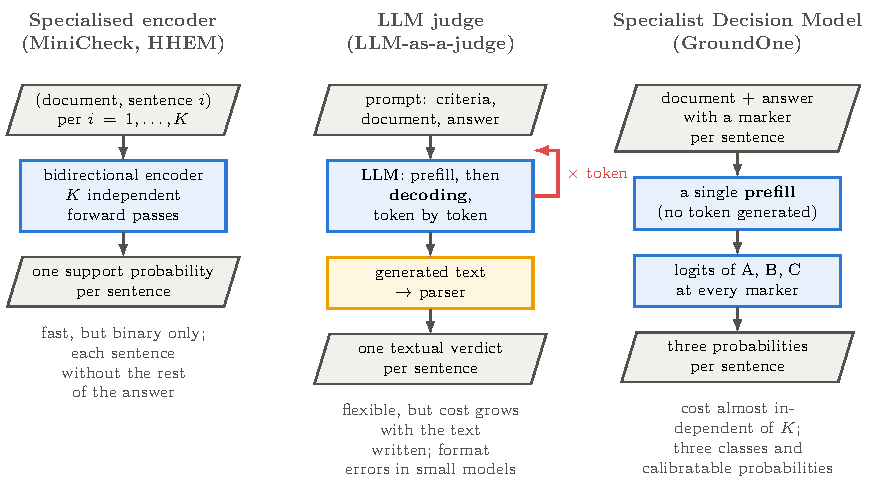
\includegraphics[width=\textwidth]{images/diagrams/bg_verifier_families_tikz.pdf}
\caption{Three ways of verifying the $K$ sentences of an answer. A specialised encoder evaluates each (document, sentence) pair in a separate forward pass and returns only a probability of support. A generative judge reads everything, but writes its verdict token by token (red loop), so its cost grows with the text produced and the output has to be interpreted by a parser. A specialist decision model reads document and answer in a single prefill and derives three probabilities from each marker, without generating any token.}
\label{fig:bg-verifiers}
\end{figure}

\section{Calibration and selective prediction}
\label{sec:bg-calibration}

A probability is calibrated when, among the predictions made with a given confidence, the fraction of correct ones
matches that confidence: in a calibrated model, for example, about 80\,\% of the predictions made with confidence 0.8
turn out to be correct.
Modern neural networks are often poorly calibrated, and a simple and effective correction is temperature scaling: the
logits are divided by a single constant, the temperature\footnote{With a temperature $T > 1$ the probabilities become
less extreme, with $T < 1$ more extreme. Since all the logits are divided by the same constant, the most probable class
does not change.}, estimated on held-out data~\cite{guo2017calibration}. The usual measure of calibration is the
Expected Calibration Error (ECE), which compares confidence and frequency of correct predictions within confidence
bins~\cite{naeini2015ece} (Section~\ref{sec:method-calibration}). For language models queried through a prompt, a
per-class bias may also be needed, to correct a systematic preference for some answers~\cite{zhao2021calibrate}.

Language models know, within limits, what they know: on closed questions, the probabilities of their tokens are often
informative about the correctness of the answer~\cite{kadavath2022know}. When the probabilities are not accessible, the
model can be asked to express its confidence in words. In large models fine-tuned with human feedback, this verbalised
confidence can be better calibrated than probabilities estimated by sampling~\cite{tian2023justask}. Systematic
evaluations, however, find it coarse and overconfident, with values concentrated on a few round
numbers~\cite{xiong2024uncertainty}.

A calibrated probability becomes useful through selective prediction: the system acts on the decisions it is confident
about and defers the others. The risk--coverage curve describes this trade-off. For each share of accepted decisions
(the coverage) it reports the error rate on them (the risk), and thus shows how the error rate falls as more decisions
are deferred~\cite{geifman2017selective}. Figure~\ref{fig:bg-risk-coverage} illustrates its typical shape.

\begin{figure}[htbp]
\centering
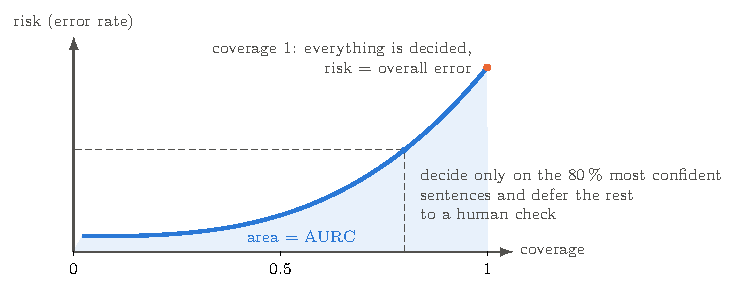
\includegraphics[width=0.75\textwidth]{images/diagrams/bg_risk_coverage_tikz.pdf}
\caption{Sketch of a risk--coverage curve (illustrative shape, not a result). The decisions are sorted from the most to the least confident; for each share decided (coverage) the error rate (risk) of the accepted decisions is reported. At coverage 1 the risk equals the overall error; giving up the least confident decisions lowers the error. The area under the curve (AURC) summarises the curve in one number: the smaller it is, the better the confidence separates correct decisions from wrong ones.}
\label{fig:bg-risk-coverage}
\end{figure}

\section{Parameter-efficient fine-tuning}
\label{sec:bg-peft}

Specialising a pre-trained model does not require updating all of its weights. Parameter-efficient fine-tuning (PEFT)
methods train only a small share of the parameters and leave the rest of the model unchanged. Low-rank adaptation (LoRA)
freezes the model and, for some weight matrices, trains only a low-rank\footnote{The \emph{rank} of a matrix is the
maximum number of its linearly independent rows (or columns). LoRA constrains the correction learned for a $d \times k$
weight matrix to have a small rank $r$. A matrix of this kind can be written as the product of two narrow matrices, one
$d \times r$ and one $r \times k$, so it suffices to store and train these two: $r(d+k)$ parameters instead of the $dk$
of the full matrix. In GroundOne 3B, for example, a $2048 \times 2048$ matrix has about 4.2 million weights, while its
rank-16 correction requires about 65 thousand, 1.6\,\%.} update. At the end of training, the update can be merged into
the weights or kept as a small separate adapter~\cite{hu2022lora}. Applying LoRA to all linear layers matters more than
using a high rank, and the technique combines with quantised base weights, so that even large models fit in little
memory~\cite{dettmers2023qlora}. The Qwen2.5 family offers open models starting from 0.5B parameters with a shared
tokenizer, and therefore makes it possible to compare different sizes with the same recipe~\cite{qwen2024qwen25}.
Figure~\ref{fig:bg-lora} sketches a LoRA adapter applied to a linear layer.

\begin{figure}[htbp]
\centering
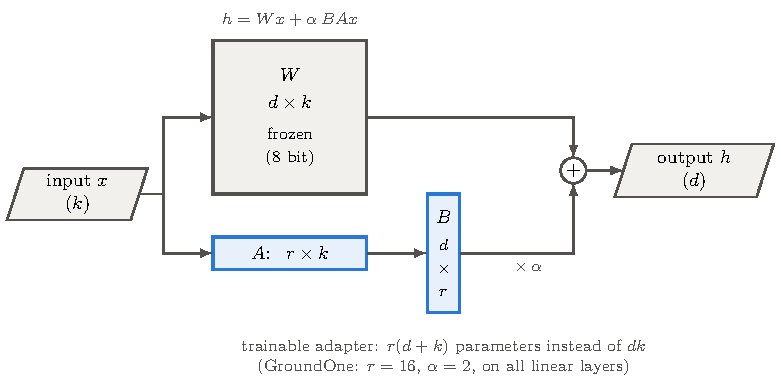
\includegraphics[width=0.8\textwidth]{images/diagrams/bg_lora_tikz.pdf}
\caption{Low-rank adaptation applied to a linear layer. The weight matrix $W$ stays frozen (8-bit in GroundOne); only the two small matrices $A$ and $B$ are trained, and their product, scaled by $\alpha$, is added to the output of the layer. With rank $r$ the adapter has $r(d+k)$ parameters instead of the $dk$ of $W$.}
\label{fig:bg-lora}
\end{figure}

Fine-tuning on small datasets, however, is notoriously unstable. Results vary with the random seed, which determines both
the initialisation of the new parameters and the order of the training data~\cite{dodge2020finetuning}. Some training
runs fail altogether, and this behaviour is linked to optimisation details such as the absence of bias correction in
Adam\footnote{Adam is an optimiser that updates each weight using two moving averages, one of the gradient and one of its
square, called moment estimates. Since these averages start from zero, in the first steps they underestimate the true
values; \emph{bias correction} rescales them to compensate. AdamW is the variant of Adam that applies weight decay
separately from the gradient.}~\cite{mosbach2021stability}. Gradient clipping, which bounds the norm of the gradient, is
finally the standard defence against occasional exploding updates~\cite{pascanu2013difficulty}.

\section{Research gap}
\label{sec:bg-gap}

The components needed for a local, fast and calibrated verifier already exist, but separately: compact open models and
runtimes that run them on a laptop, the decision-model idea of reading decisions instead of generating them, specialised
verifiers and post-hoc calibration. What is missing is an independent, controlled study that brings them together on a
single task. In particular, no work has measured whether a compact decision model, specialised in groundedness
verification, can match generative judges and dedicated encoders on this task. Nor is it known where its advantage would
come from: from specialisation, from the readout or from model size. Finally, it remains to be established whether its
probabilities are good enough to set thresholds and defer decisions, and how its time and energy compare with those of a
judge on the same consumer hardware. The rest of the thesis addresses these questions.
